\documentclass[8pt,a4paper,twoside]{tau-class/tau}
\usepackage[english]{babel}
\usepackage{stix2}
\usepackage{ctex}
\journalname{大连新东方国际教育ICC中心}
\title{CAIE 9709 − Pure Math 3 − Note}
\author[a,1]{ICC中心数学教研组}
\institution{大连新东方国际教育}
\footinfo{\LaTeX\ AQA 9665}
\theday{2025}
\leadauthor{}
\course{9709 P3}

\begin{document}

\maketitle
\tableofcontents
\linenumbers

\newpage
\section{绝对值 Absolute Value}

\subsection{绝对值的定义}
\begin{itemize}
    \item 绝对值 \(|x|\) 表示 \(x\) 到 0 的距离,始终为非负数。
    \item 例如:\(|3| = 3,\quad |−3| = 3\)。
\end{itemize}

\subsection{绝对值函数的图像}
要绘制 \(y = |ax + b|\),可以先画 \(y = ax + b\),再将 \(x\) 轴下方的部分翻折到上方。
\subsection{绝对值方程与不等式求解}
如果 \(|a| = |b|\),则 \(a = b\) 或 \(a = −b\).

\paragraph{示例:}
解方程 \(\bigl\lvert 3x − 2\bigr\rvert = 2x + 1\).
\begin{itemize}
    \item 若 \(3x − 2 \geq 0\)(即 \(x \geq \tfrac{2}{3}\)),则方程变为
    \[
        3x − 2 = 2x + 1 
        \quad \Longrightarrow \quad 
        x = 3.
    \]
    \item 若 \(3x − 2 < 0\)(即 \(x < \tfrac{2}{3}\)),则方程变为
    \[
        −(3x − 2) = 2x + 1 
        \quad \Longrightarrow \quad 
        x = \tfrac{1}{5}.
    \]
\end{itemize}
所以,解为 \(x = 3\) 或 \(x = \tfrac{1}{5}\).

\subsection{绝对值不等式的求解}
求解绝对值不等式 \(|f(x)| < a\) 或 \(|f(x)| > a\) 时,通常需要分情况讨论。

\paragraph{情况1:\(|f(x)| < a\)}
当 \(|f(x)| < a\)(其中 \(a > 0\))时,等价于
\[
    −a < f(x) < a.
\]
求解此不等式即可。

\paragraph{情况2:\(|f(x)| > a\)}
当 \(|f(x)| > a\)(其中 \(a > 0\))时,等价于
\[
    f(x) < −a \quad \text{或} \quad f(x) > a.
\]
求解两个不等式即可。

\subsubsection{形如 \(|x − a| < |x − b|\) 的不等式}
此类不等式表示点 \(x\) 到 \(a\) 的距离小于其到 \(b\) 的距离,即 \(x\) 更靠近 \(a\) 而不是 \(b\)。

\paragraph{方法 1:平方化}
由于两边均为非负数,可以平方化:
\[
    |x − a| < |x − b| \quad \Longrightarrow \quad (x − a)^2 < (x − b)^2.
\]
展开:
\[
    x^2 − 2ax + a^2 < x^2 − 2bx + b^2.
\]
消去 \(x^2\):
\[
    −2ax + a^2 < −2bx + b^2.
\]
整理:
\[
    2(b−a)x < b^2 − a^2.
\]
\[
    x < \frac{a + b}{2}, \quad \text{(当 \( a > b \))}.
\]
\[
    x > \frac{a + b}{2}, \quad \text{(当 \( a < b \))}.
\]

\paragraph{方法 2:分情况讨论}
根据绝对值的定义:
\begin{itemize}
    \item 若 \( x \geq b \),则 \(|x − a| = x − a\), \(|x − b| = x − b\),不等式变为:
    \[
        x − a < x − b.
    \]
    这个不等式始终不成立。
    \item 若 \( x \leq a \),则 \(|x − a| = a − x\), \(|x − b| = b − x\),不等式变为:
    \[
        a − x < b − x.
    \]
    这个不等式恒成立当 \( a < b \) 时。
    \item 若 \( a \leq x \leq b \),则 \(|x − a| = x − a\), \(|x − b| = b − x\),不等式变为:
    \[
        x − a < b − x.
    \]
    变形:
    \[
        2x < a + b.
    \]
    \[
        x < \frac{a + b}{2}.
    \]
\end{itemize}

因此最终解为:
\[
    x < \frac{a + b}{2}, \quad \text{(当 \( a > b \))}.
\]
\[
    x > \frac{a + b}{2}, \quad \text{(当 \( a < b \))}.
\]

\subsubsection{错误示例:平方法导致错误}
并非所有情况下都可以直接平方,错误的平方可能会改变解的范围。例如,解不等式:
\[
    |x − 3| < 2 − x.
\]

如果直接平方:
\[
    (x − 3)^2 < (2 − x)^2.
\]
展开:
\[
    x^2 − 6x + 9 < 4 − 4x + x^2.
\]
消去 \(x^2\):
\[
    −6x + 9 < 4 − 4x.
\]
整理:
\[
    −6x + 4x < 4 − 9.
\]
\[
    −2x < −5.
\]
\[
    x > \frac{5}{2}.
\]

但是,原不等式的含义是:
\[
    |x − 3| < 2 − x.
\]
当 \(2 − x < 0\)(即 \(x > 2\))时,右侧变为负数,而绝对值始终为非负数,所以整个不等式在 \(x > 2\) 时无解。

因此,我们需要分情况讨论:
\begin{itemize}
    \item 当 \( x \leq 2 \),不等式变为:
    \[
        x − 3 < 2 − x.
    \]
    \[
        2x < 5.
    \]
    \[
        x < \frac{5}{2}.
    \]
    \item 当 \( x > 2 \) 时,\( 2 − x \) 为负数,而 \( |x − 3| \) 始终非负,所以不等式无解。
\end{itemize}

最终正确解为:
\[
    x < 2.
\]

\paragraph{总结}
\begin{itemize}
    \item 绝对值不等式的解法主要有平方化和分情况讨论两种。
    \item \(|x − a| < |x − b|\) 可用平方法变形,但需注意平方后可能丢失或增加解。
    \item 直接平方时,必须确保两边非负,否则可能会导致错误的解,如 \(|x − 3| < 2 − x\) 这样的例子。
\end{itemize}
\newpage
\section{多项式除法 Polynomial Division}

可以使用长除法或综合除法(若除式是一阶多项式)来求出商与余数。

\paragraph{示例:}
用 \((x + 1)\) 除 \(x^3 − 2x^2 + x − 5\).

\begin{tcolorbox}[enhanced, breakable, boxsep=1pt, colframe=blue!50!black, colback=white, fonttitle=\footnotesize, fontupper=\footnotesize, title=长除法示意]
\centering
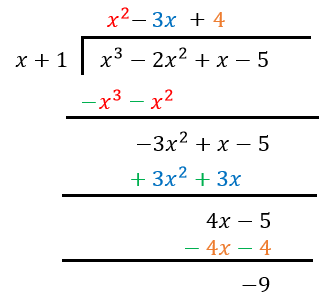
\includegraphics[width=0.65\textwidth]{long division.png}
\end{tcolorbox}

由长除法可得:
\[
    (x^3 − 2x^2 + x − 5)/(x + 1)\;=\; x^2 − 3x + 4, 
    \quad \text{余数} = −9.
\]
因此,
\[
    x^3 − 2x^2 + x − 5 
    = (x + 1)\,(x^2 − 3x + 4)\;−\;9.
\]
\section{因式定理与余数定理 Factor Theorem and Remainder Theorem}

\paragraph{因式定理(Factor Theorem):}
设 $f(x)$ 是一个多项式,且 $a$ 是某个实数。
如果 $(x − a)$ 是 $f(x)$ 的因式,那么 $f(a) = 0$。
反之,如果 $f(a) = 0$,那么 $(x − a)$ 必定是 $f(x)$ 的因式。

\paragraph{余数定理(Remainder Theorem):}
设 $f(x)$ 是一个多项式,且 $a$ 是某个实数。
当用 $f(x)$ 除以 $(x−a)$ 时,余数等于 $f(a)$。

\paragraph{示例:}
判断 $(x − 2)$ 是否是多项式 $f(x) = x^3  −  3x^2 + x + 5$ 的因式。

计算 $f(2)$:
\[
f(2) = 2^3  −  3(2^2) + 2 + 5 = 8  −  12 + 2 + 5 = 3
\]


\section{部分分式 Partial Fractions}

对于有理函数 $\frac{P(x)}{Q(x)}$,其中 $P(x)$ 为多项式,$Q(x)$ 可因式分解为一次或二次因式,可拆解为以下几种情况:

\subsection{基本形式的分解}

\paragraph{情况 1: $Q(x)$ 由互不相同的一次因子组成}

\[
    \frac{P(x)}{(ax+b)(cx+d)(ex+f)} = \frac{A}{ax+b} + \frac{B}{cx+d} + \frac{C}{ex+f}
\]

\paragraph{示例:} 分解 $\frac{2x+3}{(x+1)(x+2)}$。

设
\[
    \frac{2x+3}{(x+1)(x+2)} = \frac{A}{x+1} + \frac{B}{x+2}
\]
两边乘以分母 $(x+1)(x+2)$,得到:
\[
    2x + 3 = A(x+2) + B(x+1)
\]
展开右侧:
\[
    2x + 3 = Ax + 2A + Bx + B
\]
合并同类项:
\[
    2x + 3 = (A+B)x + (2A+B)
\]
比较系数:
\[
    A+B = 2, \quad 2A+B = 3
\]
解得 $A=1, B=1$,因此:
\[
    \frac{2x+3}{(x+1)(x+2)} = \frac{1}{x+1} + \frac{1}{x+2}
\]

\paragraph{情况 2: $Q(x)$ 具有平方因子}

\[
    \frac{P(x)}{(ax+b)(cx+d)^2} = \frac{A}{ax+b} + \frac{B}{cx+d} + \frac{C}{(cx+d)^2}
\]

\paragraph{示例:} 分解 $\frac{3x+5}{(x+1)(x+2)^2}$。

设
\[
    \frac{3x+5}{(x+1)(x+2)^2} = \frac{A}{x+1} + \frac{B}{x+2} + \frac{C}{(x+2)^2}
\]
两边乘以分母 $(x+1)(x+2)^2$,展开并比较系数求解 $A, B, C$。

\paragraph{情况 3: $Q(x)$ 含有不可因式分解的二次因子}

\[
    \frac{P(x)}{(ax+b)(cx^2+d)} = \frac{A}{ax+b} + \frac{Bx+C}{cx^2+d}
\]
\paragraph{示例:} 分解 $\frac{x^2+3x+5}{(x+1)(x^2+4)}$。

\[
    \frac{x^2+3x+5}{(x+1)(x^2+4)} = \frac{A}{x+1} + \frac{Bx+C}{x^2+4}
\]
两边乘以分母 $(x+1)(x^2+4)$,得到:
\[
x^2 + 3x + 5 = A(x^2+4) + (Bx+C)(x+1)
\]
展开右侧:
\[
A(x^2+4) + (Bx+C)(x+1) = Ax^2 + 4A + Bx^2 + Bx + Cx + C
\]
整理后:
\[
(A+B)x^2 + (B+C)x + (4A + C) = x^2 + 3x + 5
\]
比较系数:
− $x^2$ 项系数:$A + B = 1$
− $x$ 项系数:$B + C = 3$
− 常数项:$4A + C = 5$
\\
最终得到部分分式分解:
\[
\frac{x^2+3x+5}{(x+1)(x^2+4)} = \frac{3}{5(x+1)} + \frac{\frac{2}{5}x + \frac{13}{5}}{x^2+4}
\]
\newpage

\subsection{其他方法}

\begin{tcolorbox}[enhanced, breakable, boxsep=1pt, colframe=blue!50!black, colback=white, fonttitle=\footnotesize, fontupper=\footnotesize, title=求导法]
求导法可用于快速确定系数。例如,设
\[
    \frac{2x+3}{(x+1)(x+2)} = \frac{A}{x+1} + \frac{B}{x+2}
\]
两边乘以分母 $(x+1)(x+2)$ 后,对等式两边求导:
\[
    \frac{d}{dx} (2x+3) = \frac{d}{dx} \left[A(x+2) + B(x+1)\right]
\]
计算导数:
\[
    2 = A + B
\]
令 $x= − 1$ 代入原等式求 $A$:
\[
    2( − 1) + 3 = A( − 1+2) + B( − 1+1)
\]
解得 $A = 1$。

同理,令 $x= − 2$ 代入求 $B$:
\[
    2( − 2) + 3 = A( − 2+2) + B( − 2+1)
\]
解得 $B = 1$。

因此,最终结果为:
\[
    \frac{2x+3}{(x+1)(x+2)} = \frac{1}{x+1} + \frac{1}{x+2}
\]
\end{tcolorbox}

\begin{tcolorbox}[enhanced, breakable, boxsep=1pt, colframe=blue!50!black, colback=white, fonttitle=\footnotesize, fontupper=\footnotesize, title=待定系数法]
待定系数法是通用方法,即设未知数,展开等式,并通过系数比较法求解。
对于
\[
    \frac{x^2+3x+5}{(x+1)(x^2+4)} = \frac{A}{x+1} + \frac{Bx+C}{x^2+4}
\]
两边乘以分母 $(x+1)(x^2+4)$,展开等式:
\[
    x^2+3x+5 = A(x^2+4) + (Bx+C)(x+1)
\]
展开右侧:
\[
    x^2+3x+5 = Ax^2 + 4A + Bx^2 + Bx + Cx + C
\]
合并同类项:
\[
    x^2 + 3x + 5 = (A+B)x^2 + (B+C)x + (4A+C)
\]
比较系数:
\[
    A+B = 1, \quad B+C = 3, \quad 4A+C = 5
\]
解得 $A=1, B=0, C=3$。

因此,最终结果为:
\[
    \frac{x^2+3x+5}{(x+1)(x^2+4)} = \frac{1}{x+1} + \frac{3}{x^2+4}
\]
\end{tcolorbox}
\newpage
\section{指数函数与对数函数}
\subsection{指数函数与对数函数的图像}

指数函数 $y = e^x$ 和对数函数 $y = \ln x$ 互为反函数,其图像如下:

\begin{center}
    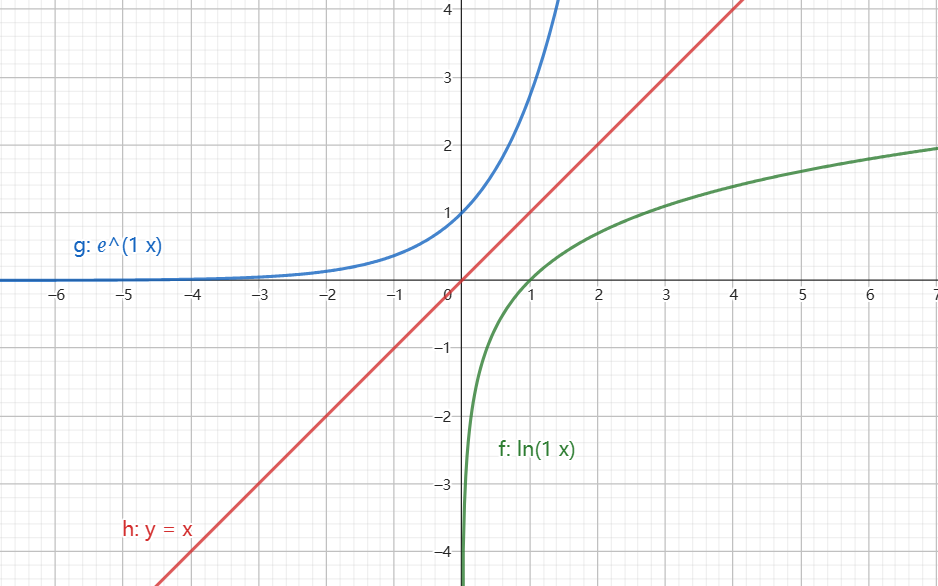
\includegraphics[width=0.45\textwidth]{figures/log and exponent.PNG}
\end{center}
\\
其中:
\begin{itemize}
    \item $y = e^x$ 在整个实数范围内定义,单调递增,过点 $(0,1)$。
    \item $y = \ln x$ 仅在 $x > 0$ 有定义,单调递增,过点 $(1,0)$。
    \item 两者关于直线 $y = x$ 对称。
\end{itemize}

\subsection{对数运算律}
对数运算的基本公式如下:
\begin{itemize}
    \item $\log_a (xy) = \log_a x + \log_a y$
    \item $\log_a \left(\frac{x}{y}\right) = \log_a x − \log_a y$
    \item $\log_a (x^n) = n \log_a x$
    \item 换底公式(考纲不要求):$\log_a b = \frac{\log_c b}{\log_c a}$
\end{itemize}

\paragraph{示例 1:指数方程求解}
解方程 $2^x = 5$。

两边取自然对数:
\[
    \ln (2^x) = \ln 5.
\]
利用对数性质 $\ln a^b = b \ln a$,得:
\[
    x \ln 2 = \ln 5.
\]
求出 $x$:
\[
    x = \frac{\ln 5}{\ln 2} \thickapprox 2.32.
\]

\paragraph{示例 2:对数不等式求解}
解不等式 $3^{2x−1} < 5^x$。

两边取自然对数:
\[
    \ln (3^{2x−1}) < \ln (5^x).
\]
利用对数性质,展开:
\[
    (2x−1) \ln 3 < x \ln 5.
\]
整理:
\[
    2x \ln 3 − x \ln 5 < \ln 3.
\]
\[
    x(2 \ln 3 − \ln 5) < \ln 3.
\]
\[
    x < \frac{\ln 3}{2 \ln 3 − \ln 5}.
\]

\subsection{对数的作用——线性化非线性关系}

\paragraph{示例 3:幂函数的线性化}
设 $y = kx^n$,对两边取自然对数:
\[
    \ln y = \ln k + n \ln x.
\]
若绘制 $\ln y$ 对 $\ln x$ 的图像,应当得到一条直线,其斜率为 $n$,截距为 $\ln k$。

\paragraph{示例 4:指数函数的线性化}
设 $y = k a^x$,对两边取自然对数:
\[
    \ln y = \ln k + x \ln a.
\]
若绘制 $\ln y$ 对 $x$ 的图像,应当得到一条直线,其斜率为 $\ln a$,截距为 $\ln k$。
\begin{tcolorbox}[enhanced, breakable, boxsep=1pt, colframe=white!50!black, colback=white, fonttitle=\footnotesize, fontupper=\footnotesize, title=Arrhenius 方程与对数线性化的应用]
A2化学中我们会学习到Arrhenius 方程,这里会是一个线性化的实际应用:
\[
k  = A e^{−\frac{E_a}{RT}}
\]
取自然对数:
\[
\ln k = \ln A − \frac{E_a}{R} \cdot \frac{1}{T}
\]
线性化后,绘制 \(\ln k\) 对 \(\frac{1}{T}\) 的图像,斜率为 \(−\frac{E_a}{R}\),可用于计算活化能 \( E_a \)。\textbf{注意:}这一方程显然数学考试不会涉及。
\end{tcolorbox}
\newpage
\subsection{指数函数 $e^x$ 的定义(极限定义)}
\textbf{考纲不做要求}。数学上 $e$ 可通过以下极限定义:
\[
    e = \lim_{n \to \text{\textit{∞}}} \left(1 + \frac{1}{n}\right)^n.
\]
更一般地,指数函数可以定义为:
\[
    e^x = \lim_{n \to \text{\textit{∞}}} \left(1 + \frac{x}{n}\right)^n.
\]
这个定义可用于推导 $e^x$ 的导数性质。
一个常见的 $e$ 的应用是\textbf{连续复利计算}。假设初始投资为 1 元,年利率为 100\%,我们考虑不同的复利方式:
\begin{tcolorbox}[enhanced, breakable, boxsep=1pt, colframe=white!50!black, colback=white, fonttitle=\footnotesize, fontupper=\footnotesize, title=连续复利计算]
\textbf{连续复利计算}。假设初始投资为 1 元,年利率为 100\%,我们考虑不同的复利方式:

- \textbf{每年复利一次}:最终金额为 \( (1 + 1)^1 = 2 \) 元。  
- \textbf{每半年复利一次}:最终金额为 \( (1 + \frac{1}{2})^2 = 2.25 \) 元。  
- \textbf{每季度复利一次}:最终金额为 \( (1 + \frac{1}{4})^4 = 2.4414 \) 元。  
- \textbf{每月复利一次}:最终金额为 \( (1 + \frac{1}{12})^{12} \thickapprox 2.613 \) 元。  
- \textbf{每周复利一次}:最终金额为 \( (1 + \frac{1}{52})^{52} \thickapprox 2.692 \) 元。  
- \textbf{每小时复利一次}:最终金额为 \( (1 + \frac{1}{8760})^{8760} \thickapprox 2.718 \) 元。  

当复利次数趋于无穷时,最终金额收敛于:
\[
\lim_{n \to \text{\textit{∞}}} \left( 1 + \frac{1}{n} \right)^n = e \thickapprox 2.718
\]
这就是  
\textbf{连续复利} 的概念,其一般公式为:
\[
A = P e^{rt}
\]
其中:
- \( P \) 为初始投资,  
- \( r \) 为年利率,  
- \( t \) 为投资年数,  
- \( A \) 为最终金额。  

\begin{center}
    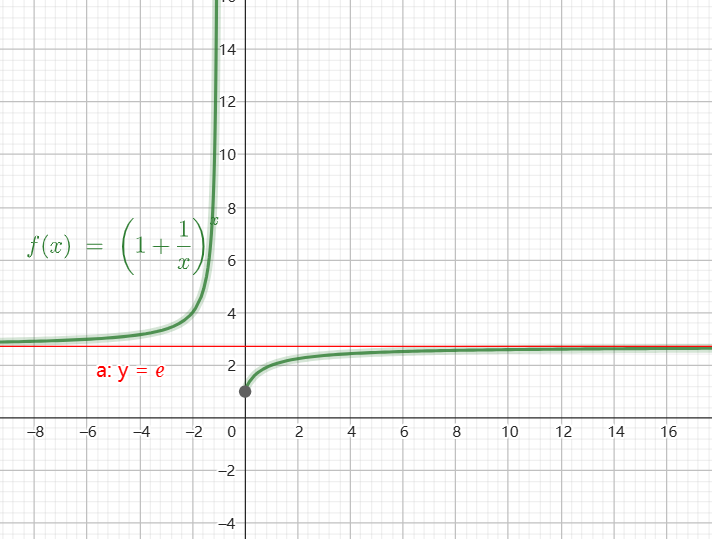
\includegraphics[width=0.8\textwidth]{figures/expoential compound interest.PNG}
\end{center}

上图展示了当复利次数 \( n \) 趋于无穷时,最终金额逐渐趋近于 \( e \)。
\end{tcolorbox}


\newpage
\section{三角函数}
\subsection{三角函数的基本关系}
三角函数之间的基本关系及图像如下如下:
\[
  \tan\theta = \frac{\sin\theta}{\cos\theta},\quad
  \cot\theta = \frac{\cos\theta}{\sin\theta},\quad
  \sec\theta = \frac{1}{\cos\theta},\quad
  \csc\theta = \frac{1}{\sin\theta}.
\]
\[
  \sin^2\theta + \cos^2\theta = 1,\quad
  1+\tan^2\theta = \sec^2\theta,\quad
  1+\cot^2\theta = \csc^2\theta.
\]

\begin{figure}[h]
    \centering
    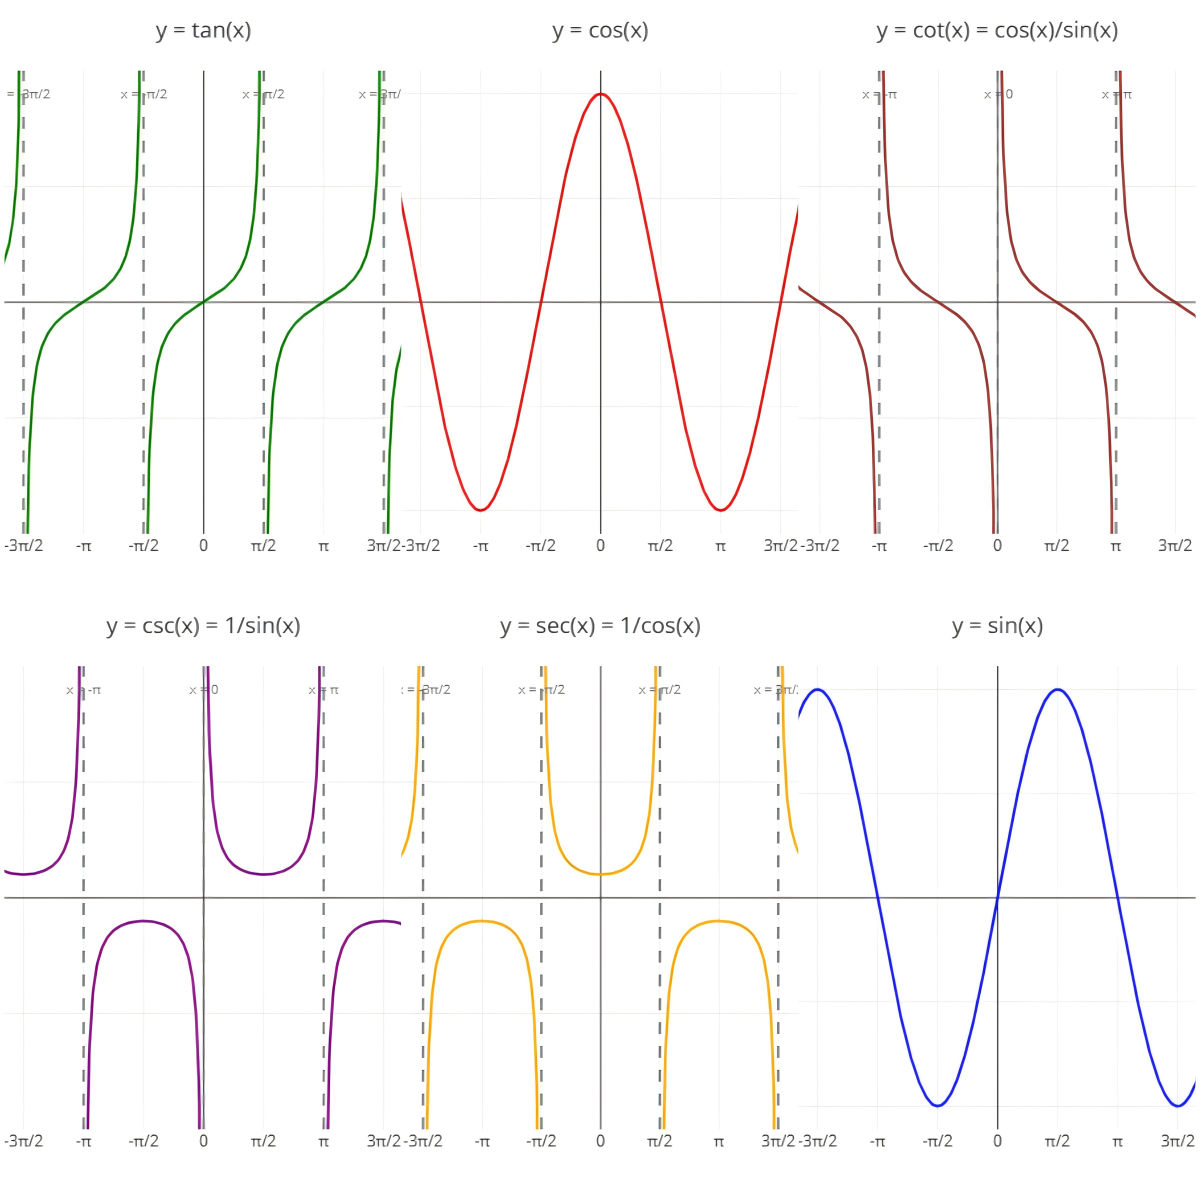
\includegraphics[width=0.45\textwidth]{figures/trig.png}
    \label{fig:trig_functions}
\end{figure}

\begin{tcolorbox}[enhanced, breakable, boxsep=1pt, colframe=blue!50!black, colback=white, fonttitle=\footnotesize, fontupper=\footnotesize, title=和差公式推导(利用欧拉公式推导考纲不做要求)]
利用欧拉公式 \(e^{i\theta}=\cos\theta+i\sin\theta\),推导:
\[
\begin{aligned}
e^{iA}e^{iB} &= e^{i(A+B)} \Rightarrow \\
(\cos A + i\sin A)(\cos B + i\sin B) &= \cos(A+B) + i\sin(A+B)
\end{aligned}
\]
比较实部和虚部,得到:
\begin{align*}
  \sin(A\pm B) &= \sin A\cos B \pm \cos A\sin B,\\[5pt]
  \cos(A\pm B) &= \cos A\cos B \mp \sin A\sin B.
\end{align*}
\end{tcolorbox}

\begin{tcolorbox}[enhanced, breakable, boxsep=1pt, colframe=blue!50!black, colback=white, fonttitle=\footnotesize, fontupper=\footnotesize, title=积化和差公式推导(利用欧拉公式推导考纲不做要求)]
利用欧拉公式 \(e^{iA}=\cos A+i\sin A\) 和 \(e^{−iA}=\cos A−i\sin A\),
\[
  e^{iA}e^{iB}+e^{−iA}e^{−iB}=2\cos(A+B),
\]
\[
  e^{iA}e^{−iB}+e^{−iA}e^{iB}=2\cos(A−B).
\]
再利用欧拉公式展开,比较实部和虚部,可得:
\begin{align*}
  \sin A\cos B &= \frac{1}{2}\Bigl[\sin(A+B)+\sin(A−B)\Bigr],\\[5pt]
  \cos A\cos B &= \frac{1}{2}\Bigl[\cos(A+B)+\cos(A−B)\Bigr],\\[5pt]
  \sin A\sin B &= \frac{1}{2}\Bigl[\cos(A−B)−\cos(A+B)\Bigr].
\end{align*}
\end{tcolorbox}

\subsection{辅助角公式}
对于表达式 \(a\sin\theta+b\cos\theta\),我们可以将其化为辅助角形式,得到两种不同的表示方法。

\paragraph{形式 1:} 令
\[
  a\sin\theta+b\cos\theta=R\sin(\theta+\phi),
\]
其中 \(R>0\) 且 \(\phi\) 为辅助角。利用和角公式,
\[
  R\sin(\theta+\phi)=R\sin\theta\cos\phi+R\cos\theta\sin\phi.
\]
比较系数得:
\[
  R\cos\phi = a,\quad R\sin\phi = b.
\]
从而,
\[
  R=\sqrt{a^2+b^2},
\]
且
\[
  \cos\phi=\frac{a}{\sqrt{a^2+b^2}},\quad \sin\phi=\frac{b}{\sqrt{a^2+b^2}}.
\]
这便得到了辅助角公式的第一种形式。

\paragraph{形式 2:} 同样,也可以写成
\[
  a\sin\theta+b\cos\theta=R\cos(\theta−\psi),
\]
其中 \(R>0\) 且 \(\psi\) 为辅助角。利用余弦差角公式,
\[
  R\cos(\theta−\psi)=R\cos\theta\cos\psi+R\sin\theta\sin\psi.
\]
比较系数得:
\[
  R\cos\psi = b,\quad R\sin\psi = a.
\]
因此,
\[
  R=\sqrt{a^2+b^2},
\]
且
\[
  \cos\psi=\frac{b}{\sqrt{a^2+b^2}},\quad \sin\psi=\frac{a}{\sqrt{a^2+b^2}}.
\]
这就是辅助角公式的第二种形式。


\subsection{三角方程求解技巧}

\paragraph{示例 1:} 解 \(\tan 2\theta=\sqrt{3}\)
\[
  2\theta=\tan^{−1}\sqrt{3}.
\]
由于 \(\tan 60^\circ=\sqrt{3}\),得到:
\[
  2\theta=60^\circ+k\cdot180^\circ.
\]
解得:
\[
  \theta=30^\circ+k\cdot90^\circ.
\]

\paragraph{示例 2:} 解 \(\sec\theta=2\)\\
利用 \(\sec\theta=\frac{1}{\cos\theta}\),得:
\[
  \cos\theta=\frac{1}{2}.
\]
查表可得:
\[
  \theta=\pm60^\circ+k\cdot360^\circ.
\]

\paragraph{示例 3:} 解 \(\cos\theta+\sin\theta=1\)\\
两边平方:
\[
  \cos^2\theta+2\cos\theta\sin\theta+\sin^2\theta=1.
\]
利用 \(\cos^2\theta+\sin^2\theta=1\),化简:
\[
  1+2\cos\theta\sin\theta=1.
\]
即 \(\sin2\theta=0\),解得:
\[
  \theta=k\cdot90^\circ.
\]

\newpage
\section{微分 Differentiation}

\subsection{求导的一般公式}
微分是研究函数变化率的重要工具,常见的求导规则如下:

\begin{tcolorbox}[enhanced, breakable, boxsep=1pt, colframe=blue!50!black, colback=white, fonttitle=\footnotesize, fontupper=\footnotesize, title=常见函数的导数]
\begin{align*}
    \frac{d}{dx} (ax^n + b) &= nax^{n−1}\quad\text{(示例: }\frac{d}{dx}(3x^4 − 2) = 12x^3\text{)},\\
    \frac{d}{dx} \ln(ax + b) &= \frac{a}{ax+b}\quad\text{(示例: }\frac{d}{dx}\ln(2x+1) = \frac{2}{2x+1}\text{)},\\
    \frac{d}{dx} e^{ax+b} &= ae^{ax+b}\quad\text{(示例: }\frac{d}{dx} e^{3x−1} = 3e^{3x−1}\text{)},\\
    \frac{d}{dx} \sin(ax+b) &= a\cos(ax+b)\quad\text{(示例: }\frac{d}{dx} \sin(5x) = 5 \cos(5x)\text{)},\\
    \frac{d}{dx} \cos(ax+b) &= −a\sin(ax+b)\quad\text{(示例: }\frac{d}{dx} \cos(x−2) = −\sin(x−2)\text{)},\\
    \frac{d}{dx} \tan^{−1}(ax) &= \frac{a}{1 + (ax)^2}\quad\text{(示例: }\frac{d}{dx} \tan^{−1}(2x) = \frac{2}{1 + 4x^2}\text{)}.
\end{align*}
\end{tcolorbox}

\subsection{链式法则(Chain Rule)}
对于复合函数 $y = f(g(x))$,求导时需要使用链式法则:
\[
    \frac{dy}{dx} = \frac{df}{dg} \cdot \frac{dg}{dx}.
\]

\begin{tcolorbox}[enhanced, breakable, boxsep=1pt, colframe=blue!50!black, colback=white, fonttitle=\footnotesize, fontupper=\footnotesize, title=链式法则: 换元法解释]
\noindent
设 $y = f\bigl(g(x)\bigr)$. 我们先令 $u = g(x)$, 则 $y = f(u)$. 通过换元:
\[
    \frac{dy}{dx} = \frac{dy}{du} \cdot \frac{du}{dx}.
\]
在具体计算时, 需要\textbf{逐层求导}, 直至最内层的 $x$ (即内层函数一直到 $1× x^1$ 为止).\\
\textbf{示例:} 计算 $\displaystyle \frac{d}{dx} \Bigl(e^{\sin (x^2 + 1)}\Bigr)$.\newline
\begin{itemize}
    \item 第 1 步: 令 $u = \sin (x^2 + 1)$, 那么 $y = e^u$.
    \item 第 2 步: $\displaystyle \frac{dy}{du} = e^u = e^{\sin(x^2+1)}$.
    \item 第 3 步: $\displaystyle \frac{du}{dx} = \cos(x^2 + 1) × 2x$, 其中 $2x$ 是继续对 $x^2 + 1$ 求导得到的最内层结果.
    \item 第 4 步: 合并:
    \[
        \frac{dy}{dx} = e^{\sin(x^2 + 1)} × \cos(x^2 + 1) × 2x.
    \]
\end{itemize}
\end{tcolorbox}

\subsection{隐函数求导 (Implicit Differentiation)}
对于隐函数 $F(x,y) = 0$, 可对两边求导并解出 $\tfrac{dy}{dx}$.

\textbf{注意:} 在隐函数求导过程中:
\begin{itemize}
  \item \textbf{等式两边对 $x$ 求导}, 即 $\tfrac{d}{dx}$ 作用于整个方程.
  \item 需要使用 \textbf{链式法则} 处理含 $y$ 的项, 因为 $y$ 是 $x$ 的函数.
\end{itemize}

\paragraph{示例 1:} 求 $x^3 + y^3 = 6xy$ 的导数.
两边对 $x$ 求导:
\[
    3x^2 + 3y^2 \frac{dy}{dx} = 6 \Bigl( x \frac{dy}{dx} + y \Bigr).
\]
整理得到:
\[
    \frac{dy}{dx} = \frac{6y − 3x^2}{3y^2 − 6x}.
\]
\paragraph{示例 2:} 若 $x^2 + y^2 = xy + 7$, 求 $\tfrac{dy}{dx}$.
\[
    2x + 2y\frac{dy}{dx} = x\frac{dy}{dx} + y.
\]
\[
    2x − y = x\frac{dy}{dx} − 2y\frac{dy}{dx} = (x − 2y)\frac{dy}{dx}.
\]
\[
    \frac{dy}{dx} = \frac{2x − y}{x − 2y}.
\]

\subsection{切线与法线求解}
切线斜率为 $m = \tfrac{dy}{dx}$, 法线斜率满足 $m_t × m_n = −1$.

\paragraph{方法 1: 直接求导求切线}
\paragraph{示例 3:} 求曲线 $x^2 + y^2 = 9$ 在 $x = 2$ 处的切线与法线方程.
隐函数求导:
\[
    2x + 2y\frac{dy}{dx} = 0 \;\Longrightarrow\; \frac{dy}{dx} = −\frac{x}{y}.
\]
代入 $x = 2$, $y = \sqrt{9 − 4} = \sqrt{5}$, 得:
\[
    m_t = −\frac{2}{\sqrt{5}}, \quad m_n = \frac{\sqrt{5}}{2}.
\]
切线方程:
\[
    y − \sqrt{5} = −\frac{2}{\sqrt{5}}(x − 2).
\]
法线方程:
\[
    y − \sqrt{5} = \frac{\sqrt{5}}{2}(x − 2).
\]

\textbf{方法 2: 联立方程, 判别式为 0}
如果方程 $F(x, y) = 0$ 不能直接求导, 可以联立 $F(x,y) = 0$ 和切线方程, 若只有一个解, 则说明该点处有唯一切线, 即判别式 $D = 0$.

\paragraph{示例 4:} 证明曲线 $y^2 = x^3 − 3x + 2$ 在某点有唯一切线.
联立 $y = mx + c$, 代入曲线方程:
\[
    (mx + c)^2 = x^3 − 3x + 2.
\]
展开整理:
\[
    x^3 − 3x + 2 − m^2x^2 − 2mcx − c^2 = 0.
\]
该方程只有一个解时, 其判别式 $D = 0$, 从而得到切线的 $m, c$ 值.

\subsection{乘积与商法则}
\paragraph{注意:}分式优先使用商法则,可以避免后续过多化简。\\
对于 $y = u(x)v(x)$, 则:
\[
    \frac{d}{dx}(uv) = u'v + uv'.
\]
\paragraph{示例 5:} $y = (x^2 + 1)(\sin x)$,
\[
    y' = 2x\,\sin x + (x^2 + 1)\,\cos x.
\]

对于 $y = \tfrac{f(x)}{g(x)}$, 则:
\[
    \left(\frac{f}{g}\right)' = \frac{g f' − f g'}{g^2}.
\]
\paragraph{示例 6:} $y = \tfrac{x^2 + 4}{x}$,
\[
    y' = \frac{x(2x) − (x^2 + 4)(1)}{x^2} = \frac{2x^2 − x^2 − 4}{x^2} = \frac{x^2 − 4}{x^2}.
\]

\subsection{参数方程求导}
若 $x = x(t), \; y = y(t)$, 则:
\[
    \frac{dy}{dx} = \frac{\frac{dy}{dt}}{\frac{dx}{dt}}.
\]
\paragraph{示例 7:} $x = t − e^{2t}, \; y = t + e^{2t}$,
\[
    \frac{dx}{dt} = 1 − 2e^{2t}, \quad \frac{dy}{dt} = 1 + 2e^{2t}, \quad \therefore \frac{dy}{dx} = \frac{1 + 2e^{2t}}{1 − 2e^{2t}}.
\]

\begin{tcolorbox}[enhanced, breakable, boxsep=1pt, colframe=blue!50!black, colback=white, fonttitle=\footnotesize, fontupper=\footnotesize, title style={align=center}, title=抛物运动(物理学中的参数方程)]
\noindent\textbf{在物理学中, 抛物运动是最常见的例子之一。} 利用参数方程, 我们可以描述物体在重力作用下的运动轨迹。设初速度为 \(v_0\) 且发射角为 \(\theta\), 则运动的参数方程为:
\[
  \begin{cases}
    x(t) = v_0\cos\theta\,t, \\[6pt]
    y(t) = v_0\sin\theta\,t − \frac{1}{2}g t^2
  \end{cases}
\]
其中 \(g\) 为重力加速度, \(t\) 为时间参数.\\[4pt]
\textit{注: 此处只是多了一个变量 \(t\). 在 A-level 的教学中, 常将导数看作分数, 因此可以直接认为}
\[
\frac{dy}{dx} = \frac{dy/dt}{dx/dt}.
\]
\textit{进一步, 由此可得}
\[
\frac{dy}{dt} = \frac{dy}{dx} \times \frac{dx}{dt},\quad \frac{dy}{dx} = \frac{1}{\frac{dx}{dy}}.
\]
通过将微分操作看作分数, 我们可以直观地进行变量替换和消约, 例如可得
\end{tcolorbox}
\begin{tcolorbox}[enhanced, breakable, boxsep=1pt, colframe=white!50!black, colback=white, fonttitle=\footnotesize, fontupper=\footnotesize, title=\textbf{证明导数的“分数”性质}]
设函数 \( f(u) \) 在 \( u = g(x) \) 处可微,且 \( g(x) \) 在 \( x \) 处可微,则复合函数
\[
h(x) = f(g(x))
\]
的导数定义为
\[
\frac{dh}{dx} = \lim_{\Delta x \to 0} \frac{f(g(x+\Delta x))−f(g(x))}{\Delta x}.
\]
对于任一 \( \Delta x\neq 0 \),由均值定理知存在 \( c \)(介于 \( g(x) \) 与 \( g(x+\Delta x) \) 之间),使得
\[
\frac{f(g(x+\Delta x))−f(g(x))}{g(x+\Delta x)−g(x)} = f'(c).
\]
因此,
\[
\frac{f(g(x+\Delta x))−f(g(x))}{\Delta x} = f'(c)\cdot \frac{g(x+\Delta x)−g(x)}{\Delta x}.
\]
取极限时,由 \( g \) 的可微性与连续性,\( c\to g(x) \),故 \( f'(c) \to f'(g(x)) \);同时,
\[
\lim_{\Delta x\to 0}\frac{g(x+\Delta x)−g(x)}{\Delta x} = g'(x).
\]
从而有
\[
\frac{dh}{dx} = f'(g(x))\cdot g'(x).
\]
以符号记号表示为
\[
\frac{dy}{dx}=\frac{dy}{du}\cdot\frac{du}{dx}.
\]
这一证明表明:尽管 \( \frac{dy}{dx} \) 本质上是一个极限,但在满足可微条件下,通过均值定理和极限运算,中间的差量 \( \Delta u \) 得以“约分”,严格地展现了类似普通分数除法的计算特性。我们注意这个其实是极限的乘法运算带来的,这一证明可以让我们非常安全的在一阶的情况下将dy/dx作为除法来使用。当然,这一部分并不做要求,大家知道就好。
\end{tcolorbox}
\newpage
\section{积分 Integration}

\subsection{基本积分及反求导}
积分是求反导数的过程。常见基本积分公式包括:
\begin{itemize}
    \item \(\displaystyle \int e^{ax+b}\,dx = \frac{1}{a}e^{ax+b} + C.\)
    \item \(\displaystyle \int \ln(ax+b)\,dx\)(通常需分部积分求解)。
    \item \(\displaystyle \int \sin(ax+b)\,dx = −\frac{1}{a}\cos(ax+b) + C.\)
    \item \(\displaystyle \int \cos(ax+b)\,dx = \frac{1}{a}\sin(ax+b) + C.\)
    \item \(\displaystyle \int \sec^2(ax+b)\,dx = \frac{1}{a}\tan(ax+b) + C.\)
    \item 多项式积分如 \(\displaystyle \int x^a\,dx = \frac{x^{a+1}}{a+1} + C\)(当 \(a\neq −1\))。
\end{itemize}

\begin{tcolorbox}[enhanced, breakable, boxsep=1pt, colframe=blue!50!black, colback=white, fonttitle=\footnotesize, fontupper=\footnotesize, title style={align=center}, title=特殊积分公式与凑微分技巧]
\noindent
对于形如
\[
\int \frac{dx}{a^2+x^2},
\]
的积分, 直接应用公式得:
\[
\int \frac{dx}{a^2+x^2} = \frac{1}{a}\tan^{−1}\Bigl(\frac{x}{a}\Bigr)+C.
\]
\textbf{凑微分技巧:} 若被积函数与标准形式仅差一个常数因子或缺少恰当的微分, 可通过乘除适当常数来凑成标准形式。\\[4pt]
\textbf{示例 1:} 计算 \(\displaystyle \int \frac{dx}{9+x^2}\).\\[4pt]
这里 \(a^2=9\) 故 \(a=3\), 应用公式得:
\[
\int \frac{dx}{9+x^2} = \frac{1}{3}\tan^{−1}\Bigl(\frac{x}{3}\Bigr)+C.
\]
\textbf{示例 2:} 计算 \(\displaystyle \int \frac{3\,dx}{9+x^2}\).\\[4pt]
提取常数后:
\[
\int \frac{3\,dx}{9+x^2} = 3\cdot \frac{1}{3}\tan^{−1}\Bigl(\frac{x}{3}\Bigr)+C = \tan^{−1}\Bigl(\frac{x}{3}\Bigr)+C.
\]
\textbf{示例 3:} 计算 \(\displaystyle \int \frac{2x}{4+x^2}\,dx\).\\[4pt]
注意到 \( \frac{d}{dx}(x^2+4)=2x\), 故令 \(u=x^2+4\), 则 \(du=2x\,dx\). 积分转化为:
\[
\int \frac{du}{u} = \ln|u|+C = \ln|x^2+4|+C.
\]
\medskip
\textbf{常用三角函数凑微分:}\\[4pt]
如果积分中出现类似 \( \frac{1}{\cos^2 \theta}\,d\theta\), 注意到
\[
\frac{d}{d\theta}(\tan \theta) = \sec^2 \theta = \frac{1}{\cos^2 \theta},
\]
故可直接令 \(u=\tan \theta\) 得 \(du = \frac{1}{\cos^2 \theta}\,d\theta\).\\[4pt]
\textbf{示例 4:} 计算 \(\displaystyle \int \frac{1}{\cos^2 \theta}\,d\theta\).\\[4pt]
直接得到:
\[
\int \frac{1}{\cos^2 \theta}\,d\theta = \tan \theta + C.
\]
\medskip
\textbf{多项式凑微分:}\\[4pt]
对于多项式凑微分, 当分子的形式正好(或几乎)是分母的导数时, 可直接凑出标准形式。\\[4pt]
\textbf{示例 5:} 计算 
\[
\int \frac{2x+1}{x^2+x+1}\,dx.
\]
注意到分母 \(x^2+x+1\) 的导数正是 \(2x+1\), 因此:
\[
\int \frac{2x+1}{x^2+x+1}\,dx = \ln\left|x^2+x+1\right|+C.
\]
\end{tcolorbox}

\subsection{三角函数积分}
为简化积分, 可利用三角恒等式和换元法。这里合并说明两种方法:

\textbf{(1) 利用三角恒等式:}\\[4pt]
例如利用倍角公式:
\[
\sin^2 x = \frac{1−\cos(2x)}{2},\quad \cos^2 x = \frac{1+\cos(2x)}{2}.
\]
\textbf{示例:} 计算 
\[
\int \sin^2 x\,dx = \int \frac{1−\cos(2x)}{2}\,dx = \frac{x}{2} − \frac{\sin(2x)}{4} + C.
\]

\textbf{(2) \(\sin^n x,\,\cos^n x,\,\tan^n x\) 的积分策略:}
\begin{itemize}
    \item 若 \(n\) 为偶数, 利用降幂公式将其转化为含双角的表达式。
    \item 若 \(n\) 为奇数, 提取单个 \(\sin x\) 或 \(\cos x\), 再利用换元法处理余下部分。
\end{itemize}
\textbf{示例 1:} 计算 
\[
\int \sin^3 x\,dx.
\]
写为:
\[
\sin^3 x = \sin x (1−\cos^2 x).
\]
令 \(u=\cos x\) (则 \(du=−\sin x\,dx\)), 得:
\[
\int \sin^3 x\,dx = −\int (1−u^2)\,du = −\cos x + \frac{\cos^3 x}{3} + C.
\]
\textbf{示例 2:} 计算 
\[
\int \tan^2 x\,dx.
\]
利用 \(\tan^2 x = \sec^2 x − 1\):
\[
\int \tan^2 x\,dx = \int (\sec^2 x−1)\,dx = \tan x − x + C.
\]

\subsection{部分分式积分}
当被积函数为有理函数时, 可先分解为部分分式, 再逐项积分. 请参照4.1部分得部分分式分解。
\paragraph{示例:}计算 
\[
\int \frac{1}{x(x+1)}\,dx.
\]
分解:
\[
\frac{1}{x(x+1)} = \frac{1}{x} − \frac{1}{x+1}.
\]
积分得:
\[
\int \frac{1}{x(x+1)}\,dx = \ln|x| − \ln|x+1| + C = \ln\left|\frac{x}{x+1}\right| + C.
\]

\subsection{分部积分 (Integration by Parts)}
积分分部公式为:
\[
\int u\,dv = uv − \int v\,du.
\]
\textbf{选取 \(u,v\) 的原则:} 按 LIATE 原则(Logarithmic, Inverse trigonometric, Algebraic, Trigonometric, Exponential)。例如对于 \(\ln x\), 取 \(u=\ln x,\; dv=dx\).
\newpage
\begin{tcolorbox}[enhanced, breakable, boxsep=1pt, colframe=blue!50!black, colback=white,
  fonttitle=\footnotesize, fontupper=\footnotesize, title style={align=center},
  title=积分分部及表格法 (Integration by Parts)]
\noindent
\textbf{积分分部公式:} \(\displaystyle \int u\,dv = uv − \int v\,du.\)\\[4pt]
\textbf{选取 \(u,v\) 的逻辑:} 按 LIATE 原则,例如对 \(\ln x\) 取 \(u=\ln x,\; dv=dx\).\\[4pt]
\textbf{表格法:} 当需要重复应用积分分部时,可用表格法整理。\\[4pt]

\textbf{示例:} 计算 \(\displaystyle \int x^2 e^{2x}\,dx\).\\[4pt]
令 \(u = x^2\)(多项式部分)与 \(dv = e^{2x}\,dx\)(指数部分)。则:
\[
\begin{cases}
  u = x^2 \quad\Rightarrow\quad du = 2x\,dx \\
  dv = e^{2x}\,dx \quad\Rightarrow\quad v = \frac{1}{2} e^{2x}
\end{cases}
\]

\noindent
\textbf{表格示意:}  
\[
\begin{array}{c|c}
  \text{D (微分)} & \text{I (积分)} \\
  \hline
  x^2 & e^{2x} \\
  2x & \tfrac{1}{2}e^{2x} \\
  2 & \tfrac{1}{4}e^{2x} \\
  0 & \tfrac{1}{8}e^{2x} \\
\end{array}
\]

\noindent
箭头交替相乘、交替加减,得到:
\[
\int x^2 e^{2x}\,dx
= \; x^2 \cdot \tfrac{1}{2} e^{2x}
− 2x \cdot \tfrac{1}{4} e^{2x}
+ 2 \cdot \tfrac{1}{8} e^{2x}
+ C.
\]

\noindent
化简可得:
\[
\int x^2 e^{2x}\,dx
= \tfrac{1}{2} x^2 e^{2x}
− \tfrac{1}{2} x\,e^{2x}
+ \tfrac{1}{4} e^{2x}
+ C.
\]
注意,这种方法(DI-method),Edexcel考局需要讲解,CAIE不做要求,CAIE也不常见复杂多项式分部积分。

\end{tcolorbox}
\subsubsection{常见隐形 "1" 形式的积分}

在积分中,常遇到形如 \(\int \ln(ax+b)\,dx\) 和 \(\int \arctan(ax+b)\,dx\) 的积分,这些积分可以看作
\[
\int 1 \cdot \ln(ax+b)\,dx \quad \text{或} \quad \int 1 \cdot \arctan(ax+b)\,dx.
\]

\paragraph{1. 积分 \(\int \ln(ax+b)\,dx\):}  
考虑积分
\[
\int \ln(ax+b)\,dx = \int 1 \cdot \ln(ax+b)\,dx.
\]
取
\[
u = \ln(ax+b), \quad dv = dx.
\]
则
\[
du = \frac{a}{ax+b}\,dx, \quad v = x.
\]
利用积分分部公式
\[
\int u\,dv = uv − \int v\,du,
\]
可得
\[
\int \ln(ax+b)\,dx = x\ln(ax+b) − \int \frac{a x}{ax+b}\,dx.
\]
注意“凑微分”:观察到
\[
\frac{x}{ax+b} = \frac{x + \tfrac{b}{a} − \tfrac{b}{a}}{ax+b} 
= \frac{1}{a} − \frac{\tfrac{b}{a}}{ax+b}.
\]
因此,
\[
\int \frac{x}{ax+b}\,dx = \frac{1}{a}\int dx − \frac{b}{a}\int \frac{dx}{ax+b}
= \frac{x}{a} − \frac{b}{a^2}\ln|ax+b| + C.
\]
代回原式得:
\[
\int \ln(ax+b)\,dx = x\ln(ax+b) − a\left(\frac{x}{a} − \frac{b}{a^2}\ln|ax+b|\right) + C,
\]
即
\[
\boxed{\int \ln(ax+b)\,dx = x\ln(ax+b) − x + \frac{b}{a}\ln|ax+b| + C.}
\]

\paragraph{示例:} 当 \(a=2\) 且 \(b=3\) 时,
\[
\int \ln(2x+3)\,dx = x\ln(2x+3) − x + \frac{3}{2}\ln|2x+3| + C.
\]

\paragraph{2. 积分 \(\int \arctan(ax+b)\,dx\):}  
同样地,将积分看作
\[
\int \arctan(ax+b)\,dx = \int 1 \cdot \arctan(ax+b)\,dx.
\]
取
\[
\textbf{令 } u = \arctan(ax+b), \quad dv = dx.
\]
则
\[
du = \frac{a}{1+(ax+b)^2}\,dx, \quad v = x.
\]
应用积分分部公式得到
\[
\int \arctan(ax+b)\,dx = x\arctan(ax+b) − \int \frac{ax}{1+(ax+b)^2}\,dx.
\]
对于 \(\int \frac{ax}{1+(ax+b)^2}\,dx\) 的进一步求解,可采用凑微分或换元法,根据具体情况处理。

\paragraph{小结:}  
凡遇到积分形如 \(\int f(x)\,dx\) 中的 \(f(x)=\ln(ax+b)\) 或 \(\arctan(ax+b)\),都可视为 \(1 \times f(x)\) 形式,然后利用积分分部法进行求解。这种“隐形的 1”的技巧在很多积分题中非常实用。




\subsection{换元法 (Substitution) 及其思路}
换元法用于将复杂积分转换为简单形式,其基本步骤为:\\
\begin{enumerate}
    \item 选取合适的代换 \(u=f(x)\), 使原积分简化。
    \item 求得 \(du = f'(x)\,dx\), 并将所有 \(x\) 的表达式转为 \(u\) 的函数。
    \item 进行积分后再换回 \(x\).
\end{enumerate}
\\
\textbf{注意:} 换元后必须利用链式法则计算 \(du/dx\) 并替换 \(dx\), 使所有被积项均用 \(u\) 表示, 最后完成积分后再换回 \(x\).\\[4pt]
\textbf{示例 1:} 计算 \(\displaystyle \int \sqrt{1−x^2}\,dx\).\\[4pt]
令 \(x=\sin \theta\) 则 \(dx=\cos \theta\,d\theta\) 且 \(\sqrt{1−x^2}=\cos \theta\). 故:
\[
\int \sqrt{1−x^2}\,dx = \int \cos \theta\cdot\cos \theta\,d\theta = \int \cos^2 \theta\,d\theta.
\]
再利用 \(\cos^2 \theta=\frac{1+\cos(2\theta)}{2}\) 继续积分.

\subsubsection{常见换元法}
\begin{tcolorbox}[enhanced, breakable, boxsep=1pt, colframe=blue!50!black, colback=white, fonttitle=\footnotesize, fontupper=\footnotesize, title style={align=center}, title=常见换元法]
\noindent
常见换元方法包括:
\begin{itemize}
    \item \textbf{根号换元:} 针对含有根号的积分, 如 \(\displaystyle \int \sqrt{1−x^2}\,dx\).\\[4pt]
    令 \(x=\sin \theta\), 则 \(dx=\cos \theta\,d\theta\) 且 \(\sqrt{1−x^2}=\cos \theta\). 积分变为 \(\int \cos^2 \theta\,d\theta\).
    \item \textbf{三角换元:} 对于包含 \(\sqrt{a^2−x^2}\), \(\sqrt{x^2+a^2}\) 或 \(\sqrt{x^2−a^2}\) 的积分, 常采用:
    \begin{itemize}
       \item 当积分含有 \(\sqrt{a^2−x^2}\) 时, 令 \(x=a\sin \theta\).
       \item 当积分含有 \(\sqrt{x^2+a^2}\) 时, 令 \(x=a\tan \theta\).
       \item 当积分含有 \(\sqrt{x^2−a^2}\) 时, 令 \(x=a\sec \theta\).
    \end{itemize}
    \item \textbf{简单代换:} 如对 \(\displaystyle \int \frac{dx}{\sqrt{x}}\), 可令 \(u=\sqrt{x}\) (则 \(x=u^2, \; dx=2u\,du\)).
\end{itemize}
\textbf{注意:} 换元后, 利用链式法则计算 \(du/dx\) 并将 \(dx\) 替换为 \(du\), 保证所有被积项均用 \(u\) 表示, 最后再换回 \(x\).
\end{tcolorbox}
\newpage
\section{数值求解方程 Numerical Solution of Equations}

\subsection{利用图形与符号变化法定位根}
一种简单而直观的方法是利用函数图形和符号变化来大致确定方程的根所在区间。\\
例如,考虑方程
\[
f(x)=x^3 − x − 2 = 0.
\]
计算得:
\[
f(1)=1^3 − 1 − 2 = 1 − 1 − 2 = −2,
\]
\[
f(2)=2^3 − 2 − 2 = 8 − 2 − 2 = 4.
\]
由于 \(f(1) < 0\) 而 \(f(2) > 0\),依据连续性定理可知,在 \(x=1\) 与 \(x=2\) 之间必有至少一个根。这种方法常用于寻找一对连续整数,使得根介于它们之间。
\subsection{示例:迭代法求根}

\paragraph{目标方程:}
我们想求解
\[
f(x) \;=\; x^3 \;−\; x \;−\; 2 \;=\; 0.
\]
题目可能已提示将此方程重排为
\[
x \;=\; \sqrt[3]{x + 2}.
\]
并给出一个初始值 \(x_0\) 以及误差限或迭代步数上限。

\paragraph{迭代步骤:}
不要求检验收敛性,但需按以下步骤逐步算出迭代值:
\begin{enumerate}
  \item \textbf{设定初值:} 例如,题目给出 \(x_0 = 1\)。
  \item \textbf{写出迭代式:}
    \[
      x_{n+1} = \sqrt[3]{x_n + 2}.
    \]
  \item \textbf{逐次迭代:} 
    \[
      x_1 = \sqrt[3]{x_0 + 2} = \sqrt[3]{1 + 2}\thickapprox 1.442,
    \]
    \[
      x_2 = \sqrt[3]{x_1 + 2} = \sqrt[3]{1.442 + 2}\thickapprox 1.515,
    \]
    \[
      x_3 = \sqrt[3]{x_2 + 2} \thickapprox \sqrt[3]{1.515 + 2}\thickapprox 1.521.
    \]
    \[
      x_4 = \sqrt[3]{x_3 + 2} \thickapprox \sqrt[3]{1.521 + 2}\thickapprox 1.522.
    \]
  \item \textbf{继续迭代:} 题目通常会给出“迭代 5 次”或“直到 \(|x_{n+1}−x_n|<10^{−3}\)”等条件。不断算下去并写出数值结果。
\end{enumerate}

\paragraph{数值结果示例:}
若重复上述过程 5~6 次,可得到下列迭代结果(保留至 3 位小数):
\[
\begin{aligned}
&x_0 = 1.000, \\
&x_1 \thickapprox 1.442,\quad x_2 \thickapprox 1.515, \\
&x_3 \thickapprox 1.521,\quad x_4 \thickapprox 1.522,\quad x_5 \thickapprox 1.522,\dots
\end{aligned}
\]
可见数值趋于约 \(1.522\).

\paragraph{说明:}
这里不要求检验是否收敛以及为什么收敛,但题目一般会保证或提示在给定形式与初值下可以完成迭代求根。

\subsection{使用 Casio fx-991 计算器进行迭代求根}
在考试中,常见的问题是利用迭代方法(Iteration Method)求根,通常题目要求的迭代步数大于 2,同时需要写出每一步的迭代结果。虽然可以手动计算,但 Casio fx-999ES 计算器的 \textbf{Spreadsheet} 功能可以帮助我们快速求解。首先,我们选择 Spreadsheet 功能(通常位于 Table 功能旁边),进入后,点击 \textbf{OPTN},选择 \textbf{Fill Formula},并输入题目给定的迭代公式。例如,本题的迭代公式为:
\[
x_{n+1} = \sqrt{4 − \sec\left(\frac{1}{2}x_n\right)}
\]
\begin{center}
    \captionsetup{labelformat=empty} 
    \fbox{
        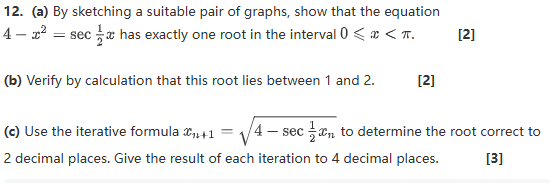
\includegraphics[width=0.48\textwidth]{figures/2022 March - 32.PNG}
    }
    \captionof{figure}{2022 March - 32}
\end{center}
需要注意计算器必须处于 \textbf{弧度模式(Radian Mode)},确保左上角显示 \textbf{R} 而不是 \textbf{D},并且在输入公式时,用 \textbf{A1} 代替 $x_n$,将 \textbf{Range} 设为 \textbf{A2:A20}(通常足够)。按下 \textbf{EXE} 运行后,迭代结果会自动填充表格,如下所示:
\begin{center}
    \includegraphics[width=0.48\textwidth]{figures/iteration method casio.png}
\end{center}
默认情况下,\textbf{A1} 的初始值为 1,若需要调整初值,例如设为 1.02,可以移动到 \textbf{A1},按 \textbf{EXE} 并输入 1.02,计算器会自动更新新的迭代结果。本题给定的范围为 $1 \leq x \leq 2$,因此可以从 1 开始。最终,我们发现结果收敛到 1.0611,取两位小数后答案为 \textbf{1.06}。最后,将 1.06 之前的迭代数据抄写到答题纸即可。
\newpage
\begin{tcolorbox}[
enhanced,
breakable,
boxsep=1pt,
colframe=blue!50!black,
colback=white,
fonttitle=\footnotesize,
fontupper=\footnotesize,
title style={align=center},
title=迭代法求根详解(Iteration Method)
]

\paragraph{一、核心原理}
\begin{itemize}[leftmargin=2em]
  \item \textbf{目标}:求解 \( f(x)=0 \) 的根(记作 \(x_0\))。
  \item \textbf{基本思想}:将原方程改写为等价的固定点形式 \( x = F(x) \),并利用迭代公式
  \[
  x_{n+1}=F(x_n),\quad n=1,2,\dots
  \]
  逐步逼近真实根 \(x_0\)。
  \item \textbf{收敛条件}:若在 \(x_0\) 附近满足
  \[
  \left|F'(x_0)\right| < 1,
  \]
  则误差以 \(\left|F'(x_0)\right|\),亦即F(x)导数 的比例缩小,从而收敛。
\end{itemize}

\paragraph{二、收敛条件详细解析}
\begin{itemize}[leftmargin=2em]
  \item 令误差 \(e_n=x_n − x_0\),在 \(x_0\) 附近对 \(F(x_n)\) 展开:
    \[
    F(x_n)=F(x_0+e_n)\thickapprox F(x_0)+F'(x_0)e_n.
    \]
    由于 \(F(x_0)=x_0\),可得
    \[
    x_{n+1}=F(x_n)\thickapprox x_0+F'(x_0)e_n.
    \]
    因此,新误差为:
    \[
    e_{n+1}\thickapprox F'(x_0)e_n.
    \]
    若 \(\left|F'(x_0)\right|<1\),误差递减,保证收敛。

  \item \textbf{数值示例}:设
    \[
    F(x)=\frac{1}{2}x+1.
    \]
    \textbf{求固定点}:
    \[
    x_0=\frac{1}{2}x_0+1 \quad\Rightarrow\quad x_0=2.
    \]
    \textbf{计算导数}:
    \[
    F'(x)=\frac{1}{2},\quad \left|F'(2)\right|=\frac{1}{2}<1.
    \]
    \textbf{取初值 \(x_1=0\),进行迭代}:
    \begin{align*}
      x_2 &= \frac{1}{2} \cdot 0 +1 =1, \\
      x_3 &= \frac{1}{2} \cdot 1 +1 =1.5, \\
      x_4 &= \frac{1}{2} \cdot 1.5 +1 =1.75, \\
      x_5 &= \frac{1}{2} \cdot 1.75 +1 =1.875.
    \end{align*}
    \textbf{观察误差}:
    \[
    \begin{array}{r l}
        e_1 &= 0 − 2 = −2, \\
        e_2 &= 1 − 2 = −1, \\
        e_3 &= 1.5 − 2 = −0.5, \\
        e_4 &= 1.75 − 2 = −0.25.
    \end{array}
    \]
    可见每步误差均约缩小一半,与 \(\left|F'(2)\right| = \frac{1}{2}\) 的比例一致。
\end{itemize}


\paragraph{四、总结}
\begin{itemize}[leftmargin=2em]
  
  \begin{itemize}
    \item 收敛条件:\(\left|F'(x_0)\right|<1\) 保证误差缩小,使得 \(x_n\) 收敛到 \(x_0\)。
    \item P3题目一般会在第一问或者第二问给出x=F(x),直接迭代;后期考试(如 Further Math或者入学考试)会考察用导数来逼近函数值的思路。这个也是泰勒展开的核心思路。
  \end{itemize}
\end{itemize}

\end{tcolorbox}
\newpage



\subsection{利用计算器表格功能辅助求根}
\paragraph{}
在实际应用中,可以利用计算器(如 Casio fx-991EX)的表格功能来辅助定位根。输入函数
\[
f(x)=x^3 − x − 2,
\]
并生成一系列 \(x\) 值对应的 \(f(x)\) 值,观察符号变化即可确定根所在的区间。\\[4pt]
例如,当 \(x\) 从 1 到 2,步长为 0.1 时,可能得到如下表格:
\[
\begin{array}{c|c}
x & f(x) \\ \hline
1.0 & −2.0 \\
1.1 & −1.37 \\
1.2 & −0.73 \\
1.3 & −0.07 \\
1.4 & 0.59 \\
1.5 & 1.13 \\
\end{array}
\]
从表中可见,在 \(x \thickapprox 1.3\) 附近 \(f(x)\) 由负变正,因此根位于该区间。\\[4pt]
下图为 Casio fx-991EX 计算器表格功能的截图示例:
\begin{center}
\includegraphics[width=0.5\textwidth]{casio_table.png}
\end{center}
\begin{tcolorbox}[enhanced, breakable, boxsep=1pt, colframe=blue!50!black, colback=white, fonttitle=\footnotesize, fontupper=\footnotesize, title style={align=center}, title=计算器表格功能使用说明]
首先,按计算器的 Mode 选择 Table 功能。选择完毕后,输入方程。例如,输入 \(f(x)=x^3−x−2\)。
\\[4pt]
通常题目会给出参考值,设定 Start 和 End 值,然后根据题目要求设置步长(Step),并调整小数点位数。\\[4pt]
在表格中,当我们观察到某一行 \(f(x_1) < 0\) 而下一行 \(f(x_2) > 0\) 时,即可判定根存在于 \(x_1\) 与 \(x_2\) 之间。
\end{tcolorbox}
\newpage
\section{Vectors}

\subsection{标准记号与表示法}

\paragraph{向量的本质:大小与方向}
向量可以被视为“既有大小又有方向的量”。只要\textbf{长度相等}且\textbf{方向相同},两个向量就被称为\textbf{相等},即便它们在坐标平面中并不“重叠”。

\paragraph{位置向量 (Position Vector) vs. 位移向量 (Displacement Vector)}
\begin{itemize}
  \item \textbf{位置向量}: 当我们将原点 \(O\) 作为公共起点,用向量 \(\overrightarrow{OA}\) 表示点 \(A\) 的位置,这个向量的起点固定在 \(O\),其大小与方向决定了 \(A\) 在坐标系中的位置。
  \item \textbf{位移向量}: 更一般地,若从点 \(P\) 到点 \(Q\) 的向量记为 \(\overrightarrow{PQ}\),这是一个\textit{位移},不一定以原点开头。只要大小和方向相同,即使它们起点不同,这些向量在数学上依然“相等”。
\end{itemize}

\paragraph{示例:}
若 \(O=(0,0)\),\(A=(1,2)\),则
\[
\overrightarrow{OA} = \begin{pmatrix}1\\2\end{pmatrix}.
\]
若再令 \(B=(2,4)\),则
\[
\overrightarrow{AB}=\begin{pmatrix}2−1\\4−2\end{pmatrix}
=\begin{pmatrix}1\\2\end{pmatrix}.
\]
因此 \(\overrightarrow{OA}\) 与 \(\overrightarrow{AB}\) 方向相同、长度相同,视为“相等向量”,即使它们并不重叠。

\paragraph{向量的坐标表示}
- 在二维:
\[
\text{竖向量: } \begin{pmatrix} x\\[4pt] y\end{pmatrix}, 
\qquad
\text{或 }
x\mathbf{i}+y\mathbf{j}.
\]
- 在三维:
\[
\begin{pmatrix} x\\[2pt] y\\[2pt] z\end{pmatrix},
\qquad
x\mathbf{i}+y\mathbf{j}+z\mathbf{k}.
\]

\paragraph{向量大小 (Length / Magnitude)}
- 二维向量 \(\mathbf{u} = \begin{pmatrix}u_1\\u_2\end{pmatrix}\) 的长度为
\[
\|\mathbf{u}\| = \sqrt{u_1^2 + u_2^2}.
\]
- 三维向量 \(\mathbf{v} = \begin{pmatrix}v_1\\v_2\\v_3\end{pmatrix}\) 的长度为
\[
\|\mathbf{v}\| = \sqrt{v_1^2 + v_2^2 + v_3^2}.
\]
同理,如果用 \(\mathbf{i},\mathbf{j},\mathbf{k}\) 表示,则 \(\mathbf{u} = u_1\mathbf{i} + u_2\mathbf{j}\) 时长度为 \(\sqrt{u_1^2 + u_2^2}\),三维情形多一个 \(u_3\mathbf{k}\) 即可。

\subsection{向量的加减与数乘}

给定二维向量 
\(\mathbf{u}=\begin{pmatrix}u_1\\[2pt]u_2\end{pmatrix}\)
和
\(\mathbf{v}=\begin{pmatrix}v_1\\[2pt]v_2\end{pmatrix}\),
则加法、减法如下:
\[
\mathbf{u} + \mathbf{v}
= \begin{pmatrix}u_1+v_1\\u_2+v_2\end{pmatrix},
\quad
\mathbf{u} − \mathbf{v}
= \begin{pmatrix}u_1 − v_1\\u_2 \subsection{按比例分点:\(AB : BC = 1 : n\)}

假设点 \(A\)、\(B\)、\(C\) 共线,且 \(B\) 在 \(A\) 与 \(C\) 之间,使
\[
AB : BC \;=\; 1 : n.
\]
如果我们用 \(\mathbf{a}, \mathbf{b}, \mathbf{c}\) 分别表示点 \(A,B,C\) 的\textbf{位置向量}(即从原点 \(O\) 到这些点的向量),则要找 \(\mathbf{b}\) 满足上述比例关系。

\paragraph{结论:}
若 \(\overrightarrow{OA}=\mathbf{a}\) 与 \(\overrightarrow{OC}=\mathbf{c}\),并且 \(B\) 为将线段 \(AC\) 内部分成 \(1:n\) 的点,则
\[
\mathbf{b} \;=\; \overrightarrow{OB}
\;=\;
\frac{\,\mathbf{c} \;+\; n\,\mathbf{a}\,}{\,1 + n\,}.
\]
换言之,\(B\) 的位置向量是 \(\mathbf{c}\) 与 \(\mathbf{a}\) 的适当线性组合。

\paragraph{原理说明:}
\begin{itemize}
  \item 设整段 \(AC\) 分为“1 + n” 份,其中 \(AB\) 占 1 份,\(BC\) 占 \(n\) 份。
  \item 由向量思路可写 
    \[
      \overrightarrow{AB} 
      = \overrightarrow{OB} − \overrightarrow{OA}
      = \mathbf{b} − \mathbf{a},
      \quad
      \overrightarrow{BC}
      = \mathbf{c} − \mathbf{b}.
    \]
  \item 由比率 \(AB:BC=1:n\),可推出
    \(\overrightarrow{AB} = \tfrac{1}{n}\overrightarrow{BC}\) 或结合 \(\overrightarrow{AC} = \overrightarrow{AB} + \overrightarrow{BC}\) 等关系,整理即可得
    \[
      \mathbf{b} = \frac{\mathbf{c} + n\,\mathbf{a}}{1+n}.
    \]
\end{itemize}

\paragraph{示例:}
在二维中,若 \(A=(0,0)\) 与 \(C=(4,0)\)(位置向量分别 \(\mathbf{a}=\langle 0,0\rangle\), \(\mathbf{c}=\langle 4,0\rangle\)),且要求 \(AB:BC=1:3\)。则
\[
\mathbf{b}
= \frac{\mathbf{c} + 3\mathbf{a}}{1+3}
= \frac{\langle 4,0\rangle + 3\langle 0,0\rangle}{4}
= \frac{\langle 4,0\rangle}{4}
= \langle 1,0\rangle.
\]
因此 \(B\) 在平面坐标中为 \((1,0)\),把段 \(AC\) 划分成“1 比 3”的内部点。

\paragraph{位置向量与比例分点:}
− 这里的 \(\mathbf{a}=\overrightarrow{OA}\)、\(\mathbf{c}=\overrightarrow{OC}\),均是“从原点 \(O\)”出发的\textbf{位置向量}。
− \(\mathbf{b}=\overrightarrow{OB}\) 亦是\textbf{位置向量},但要满足在同一直线上分割线段 \(AC\) 的比例条件。
− 这一公式(有时也叫“内分点公式”)是位置向量应用的重要实例:即**分割线段**所处点的坐标可通过线性组合得出。
 v_2\end{pmatrix}.
\]
若 \(\lambda\) 是一个实标量,则数乘
\[
\lambda\,\mathbf{u}
= \begin{pmatrix}\lambda\,u_1\\ \lambda\,u_2\end{pmatrix}.
\]

\paragraph{平行四边形法则:}
向量相加可用“平行四边形法则”来理解:从同一起点作出 \(\mathbf{u}\) 和 \(\mathbf{v}\),\(\mathbf{u}+\mathbf{v}\) 对应该平行四边形的一条对角线。

\paragraph{示例:}
若
\(\mathbf{u}=\begin{pmatrix}2\\3\end{pmatrix}\),
\(\mathbf{v}=\begin{pmatrix}−1\\4\end{pmatrix}\),
则
\[
\mathbf{u}+\mathbf{v}
= \begin{pmatrix}2+(−1)\\3+4\end{pmatrix}
= \begin{pmatrix}1\\7\end{pmatrix}.
\]

\begin{tcolorbox}[enhanced, breakable, boxsep=1pt, colframe=blue!50!black, colback=white,
  fonttitle=\footnotesize, fontupper=\footnotesize, title style={align=center},
  title=物理中的向量: 方向与大小]
\paragraph{单位向量 \(\hat{\mathbf{u}}\):}
给定非零向量 \(\mathbf{u}\),其单位向量定义为
\[
\hat{\mathbf{u}} = \frac{\mathbf{u}}{\|\mathbf{u}\|},
\]
即“提取向量的方向”。若需大小为 \(M\) 的向量与 \(\mathbf{u}\) 同方向,则可写
\[
M \cdot \hat{\mathbf{u}}
= M \cdot \frac{\mathbf{u}}{\|\mathbf{u}\|}
= \frac{M}{\|\mathbf{u}\|}\mathbf{u}.
\]

\paragraph{示例(速度向量):}
若在物理中某物体速度方向给出为 \(\begin{pmatrix}2\\3\\4\end{pmatrix}\),而希望速度大小为 100,则先算其长度
\[
\|\mathbf{d}\|
= \sqrt{2^2 + 3^2 + 4^2}
= \sqrt{29}.
\]
单位向量为
\[
\hat{\mathbf{d}} = \frac{1}{\sqrt{29}}\begin{pmatrix}2\\3\\4\end{pmatrix}.
\]
故实际速度向量可写为
\[
\mathbf{v} = 100\;\hat{\mathbf{d}}
= \frac{100}{\sqrt{29}} \begin{pmatrix}2\\3\\4\end{pmatrix},
\]
实现了“大小为 100,方向与 \(\begin{pmatrix}2,3,4\end{pmatrix}\) 相同”。
\end{tcolorbox}

\begin{tcolorbox}[enhanced, breakable, boxsep=1pt, colframe=blue!50!black, colback=white,
  fonttitle=\footnotesize, fontupper=\footnotesize, title style={align=center},
  title=用向量描述平面变换 (Translation)]
\paragraph{平移 (Translation)}
在 2D 中,\textbf{平移}可由某个向量 \(\mathbf{t}\) 表示:
\[
\mathbf{v} \;\mapsto\; \mathbf{v} + \mathbf{t}.
\]
例如,要把所有点向右 2、向上 1,则可令
\[
\mathbf{t}=\begin{pmatrix}2\\1\end{pmatrix},
\]
则对任意点(或向量坐标)\(\mathbf{v}=\begin{pmatrix}x\\y\end{pmatrix}\),平移后得到新的坐标
\[
\begin{pmatrix}x\\y\end{pmatrix} \;\mapsto\; \begin{pmatrix}x\\y\end{pmatrix} + \begin{pmatrix}2\\1\end{pmatrix}
= \begin{pmatrix}x+2\\ y+1\end{pmatrix}.
\]
\end{tcolorbox}



\subsection{直线的方程:\(\mathbf{r} = \mathbf{a} + t\,\mathbf{b}\)}
\paragraph{}
在 2D 或 3D 空间中,一条直线可写作
\[
\mathbf{r} = \mathbf{a} + t\,\mathbf{b},
\]
其中:
\begin{itemize}
    \item \(\mathbf{r}\) 是直线上任意点的\textbf{位置向量};
    \item \(\mathbf{a}\) 是直线上某已知点(参考点)的位置向量;
    \item \(\mathbf{b}\) 是直线的\textbf{方向向量};
    \item \(t\) 是实数参数。
\end{itemize}
\paragraph{示例:}
若已知直线上两点 \(P\) 和 \(Q\),其位置向量分别为 \(\mathbf{p}\) 和 \(\mathbf{q}\),则直线可写为
\[
\mathbf{r} = \mathbf{p} + t\,(\mathbf{q}−\mathbf{p}),
\]
其中 \(\mathbf{q}−\mathbf{p}\) 即方向向量。

\subsection{直线间的关系:平行、相交或异面 (skew)}
\paragraph{}
给定两条直线:
\[
\mathbf{r} = \mathbf{a} + \lambda\,\mathbf{b}
\quad\text{与}\quad
\mathbf{r} = \mathbf{c} + \mu\,\mathbf{d}.
\]
\begin{itemize}
    \item \textbf{平行:} 若 \(\mathbf{b}\) 与 \(\mathbf{d}\) 互为标量倍数,即 \(\mathbf{b} = k\,\mathbf{d}\),则两线平行或重合。
    \item \textbf{相交:} 若存在 \(\lambda,\mu\) 使得 \(\mathbf{a} + \lambda\,\mathbf{b} = \mathbf{c} + \mu\,\mathbf{d}\),则两线相交,可解出交点坐标。
    \item \textbf{异面:} 若既不平行也无公共点,则称为\textbf{异面直线}(skew lines)。(考纲不要求计算两异面直线的最短距离或公垂线。)
\end{itemize}

\subsection{标量积(点积)与应用}
\paragraph{}
两个向量 \(\mathbf{u},\mathbf{v}\) 的标量积(点积)定义为
\[
\mathbf{u}\cdot\mathbf{v} = \|\mathbf{u}\|\;\|\mathbf{v}\|\;\cos\theta,
\]
其中 \(\theta\) 是 \(\mathbf{u}\) 与 \(\mathbf{v}\) 之间的夹角。坐标形式下,
\[
\langle u_1,\,u_2\rangle \cdot \langle v_1,\,v_2\rangle = u_1v_1 + u_2v_2
\]
(3D 类似,加上 \(u_3v_3\)).\\[4pt]
\paragraph{几何应用:}
\begin{itemize}
    \item \textbf{求两直线夹角:} 若线 \(\ell_1\) 与 \(\ell_2\) 的方向向量分别为 \(\mathbf{b}\) 与 \(\mathbf{d}\),则它们夹角 \(\phi\) 满足
    \[
    \cos \phi = \frac{\mathbf{b}\cdot \mathbf{d}}{\|\mathbf{b}\|\;\|\mathbf{d}\|}.
    \]
    \item \textbf{垂直条件:} \(\mathbf{u}\perp \mathbf{v}\) 当且仅当 \(\mathbf{u}\cdot \mathbf{v}=0\).
    \item \textbf{投影与垂足:} 若求某点到一条线的垂足,也可利用标量积方程组进行求解。
\end{itemize}
\paragraph{示例:}
若有向量 \(\mathbf{u}=\langle 1,2,3\rangle\)、\(\mathbf{v}=\langle 2,1,−1\rangle\),则
\[
\mathbf{u}\cdot\mathbf{v} = 1\times 2 + 2\times 1 + 3\times (−1) = 2+2−3=1.
\]
由此可知 \(\mathbf{u}\) 与 \(\mathbf{v}\) 之间的夹角 \(\theta\) 满足
\[
\cos\theta = \frac{1}{\sqrt{1^2+2^2+3^2}\;\sqrt{2^2+1^2+(−1)^2}} = \frac{1}{\sqrt{14}\;\sqrt{6}}.
\]

\subsection{总结}
\\
\paragraph{}
\begin{itemize}
    \item \textbf{向量表示:} 2D 时 \(\langle x,y\rangle\)、3D 时 \(\langle x,y,z\rangle\),或用 \(\mathbf{i},\mathbf{j},\mathbf{k}\).
    \item \textbf{运算:} 向量加减、数乘、求模、单位向量等几何解释。
    \item \textbf{位置向量:} 原点 \(O\) 到点 \(A\) 的向量 \(\overrightarrow{OA}\);中点及平行四边形等用位置向量表示。
    \item \textbf{直线方程:} \(\mathbf{r}=\mathbf{a}+t\,\mathbf{b}\);检查两线平行、相交或异面。
    \item \textbf{标量积:} \(\mathbf{u}\cdot\mathbf{v}=\|\mathbf{u}\|\|\mathbf{v}\|\cos\theta\),用于判断垂直、求夹角、求垂足等。
\end{itemize}
\textbf{不要求:} 矢量积、异面直线最短距离、公垂线。
\subsection{按比例分点:\(AB : BC = 1 : n\)}

假设点 \(A\)、\(B\)、\(C\) 共线,且 \(B\) 在 \(A\) 与 \(C\) 之间,使
\[
AB : BC \;=\; 1 : n.
\]
如果我们用 \(\mathbf{a}, \mathbf{b}, \mathbf{c}\) 分别表示点 \(A,B,C\) 的\textbf{位置向量}(即从原点 \(O\) 到这些点的向量),则要找 \(\mathbf{b}\) 满足上述比例关系。

\paragraph{结论:}
若 \(\overrightarrow{OA}=\mathbf{a}\) 与 \(\overrightarrow{OC}=\mathbf{c}\),并且 \(B\) 为将线段 \(AC\) 内部分成 \(1:n\) 的点,则
\[
\mathbf{b} \;=\; \overrightarrow{OB}
\;=\;
\frac{\,\mathbf{c} \;+\; n\,\mathbf{a}\,}{\,1 + n\,}.
\]
换言之,\(B\) 的位置向量是 \(\mathbf{c}\) 与 \(\mathbf{a}\) 的适当线性组合。

\paragraph{原理说明:}
\begin{itemize}
  \item 设整段 \(AC\) 分为“1 + n” 份,其中 \(AB\) 占 1 份,\(BC\) 占 \(n\) 份。
  \item 由向量思路可写 
    \[
      \overrightarrow{AB} 
      = \overrightarrow{OB} − \overrightarrow{OA}
      = \mathbf{b} − \mathbf{a},
      \quad
      \overrightarrow{BC}
      = \mathbf{c} − \mathbf{b}.
    \]
  \item 由比率 \(AB:BC=1:n\),可推出
    \(\overrightarrow{AB} = \tfrac{1}{n}\overrightarrow{BC}\) 或结合 \(\overrightarrow{AC} = \overrightarrow{AB} + \overrightarrow{BC}\) 等关系,整理即可得
    \[
      \mathbf{b} = \frac{\mathbf{c} + n\,\mathbf{a}}{1+n}.
    \]
\end{itemize}

\paragraph{示例:}
在二维中,若 \(A=(0,0)\) 与 \(C=(4,0)\)(位置向量分别 \(\mathbf{a}=\langle 0,0\rangle\), \(\mathbf{c}=\langle 4,0\rangle\)),且要求 \(AB:BC=1:3\)。则
\[
\mathbf{b}
= \frac{\mathbf{c} + 3\mathbf{a}}{1+3}
= \frac{\langle 4,0\rangle + 3\langle 0,0\rangle}{4}
= \frac{\langle 4,0\rangle}{4}
= \langle 1,0\rangle.
\]
因此 \(B\) 在平面坐标中为 \((1,0)\),把段 \(AC\) 划分成“1 比 3”的内部点。

\paragraph{位置向量与比例分点:}
− 这里的 \(\mathbf{a}=\overrightarrow{OA}\)、\(\mathbf{c}=\overrightarrow{OC}\),均是“从原点 \(O\)”出发的\textbf{位置向量}。
− \(\mathbf{b}=\overrightarrow{OB}\) 亦是\textbf{位置向量},但要满足在同一直线上分割线段 \(AC\) 的比例条件。
− 这一公式(有时也叫“内分点公式”)是位置向量应用的重要实例:即**分割线段**所处点的坐标可通过线性组合得出。





\end{document}
